\part{Mecánica Clásica}

\vspace*{\fill}

\begin{center}
	\textit{''La frase más exitante que se puede oír en ciencia, la que anuncia nuevos descubrimientos, no es «eureka» sino «Eso es divertido...»'' - Isaac Asimov.}
\end{center}

\vspace*{\fill}

\chapter{Movimiento de una Partícula en una Dimensión}

Se estudiará el movimiento de una partícula a lo largo de una línea recta.

\section{Teoremas de Energía y Momentum}
El movimiento de una partícula esta gobernado por la ecuación de la Segunda Ley de Newton
\begin{equation}
	F = m\dv[2]{x}{t}.
\end{equation}

Antes de considerar su solución de esta ecuación es necesario recordar algunos conceptos básicos, como el momentum lineal
\begin{equation}
	p = mv = m\dv{x}{t}.
\end{equation}

Suponiendo que la masa es constante (esto no es cierto en casos específicos), se tiene

\begin{equation}
	F = \dv{p}{t}.
\end{equation}

Esta ecuación muestra que el cambio del momentum en el tiempo es igual a la fuerza aplicada. A esto le llamammos el Teorema del Momentum Lineal. Integrando en el tiempo, se tiene 
\begin{equation}
	p_2 - p_1 = \int _{t_1} ^{t_2} F \dd{t}.
\end{equation}

A la integral de la derecha se le conoce como \textit{Impulso}. \\


Otra cantidad importante a tomar en cuenta es la \textit{energía cinética}
\begin{equation}
	T = \frac{1}{2} mv^2.
\end{equation}

Multiplicando la Segunda Ley de Newton por la velocidad, se tiene lo siguiente
\begin{equation}
	\dv{t} \qty(\frac{1}{2} mv^2) = \dv{T}{t} = Fv.
\end{equation}
Integrando de ambos lados y reemplazando la velocidad por su definición, se llega al \textit{Teorema Trabajo y Energía}

\begin{equation}
	T_2 - T_1 = \int _{t_1} ^{t_2} F \dd{x}.
\end{equation}

\section{Fuerza}

\subsection{Fuerza Aplicada Dependiente del Tiempo}

SI la fuerza $F$ está dada por una función dependiente del tiempo, resolviendo el teorema impulso momento para $x$ y $\dot{x}$.
\begin{align}
	v &= v_o + \frac{1}{m} \int _{t_o} ^t F(t) \dd{t} \\
	x - x_o &= v_o (t - t_o) + \frac{1}{m} \int _{t_o} ^t \qty[\int _{t_o} ^t F(t) \dd{t}] \dd{t} .
\end{align}


\subsection{Fuerza de Restitución Dependiente de la Velocidad}
La Segunda Ley de Newton en términos de la velocidad
\begin{equation}
	m\dv{v}{t} = F(v).
\end{equation}
Integramos y se obtienen soluciones de la siguiente forma
\begin{align*}
	v &= \varphi \qty(v_o , \frac{t - t_o}{m}) \\
	x &= x_o + \int _{t_o} ^t \varphi \qty(v_o , \frac{t - t_o}{m}) \dd{t}.
\end{align*}
Estas fuerzas restitutivas dependen de potencias de la velocidad del objeto/sistema en movimiento 
	\begin{equation}
		F = \mp bv^n,
	\end{equation}
Si $n$ es un entero impar, se toma el signo negativo, en otro caso se toma el signo de modo que la velocidad sea opuesta a la velocidad.

\subsection{Fuerza Conservativa}

Para una fuerza dependiente exclusivamente de la posición. Ahora definimos la energía potencial
\begin{equation}
	V(x) = - \int _{x_s} ^x F(x) \dd{x}
\end{equation}
Con esto se puede definir la energía total
\begin{equation}
	E = T + V.
\end{equation}
Resolviendo para la velocidad se obtiene
\begin{equation}
	v = \dv{x}{t} = \sqrt{\frac{2}{m}} \qty[E - V(x)]^{1/2}
\end{equation}
entonces
\begin{equation}
	\sqrt{\frac{m}{2}} \int _{x_o} ^x \qty[E - V(x)]^{1/2} \dd{x} = t - t_o.
\end{equation}
Con todo esto obtenemos la relación directa entre potencial y fuerza
\begin{equation}
	F = -\grad{V}
\end{equation}

\subsubsection{Campos Vectoriales}
Para que un campo vectorial $\vec{F}$ sea considerado conservativo, deben cumplirse las siguientes condiciones:

\begin{enumerate}
    \item \textbf{Existencia de un potencial escalar:} Existe una función escalar $f$ tal que $\vec{F} = \nabla f$. Esto significa que el campo vectorial puede ser expresado como el gradiente de una función escalar.
    
    \item \textbf{La circulación de $\vec{F}$ sobre cualquier curva cerrada es cero:} Para que un campo vectorial $\vec{F}$ sea conservativo, la integral de línea del campo vectorial sobre cualquier curva cerrada $C$ debe ser cero:
    $$
    \oint_{C} \vec{F} \cdot d\vec{r} = 0
    $$
    Esto implica que el trabajo realizado por el campo a lo largo de una trayectoria cerrada es nulo.
    
    \item \textbf{Independencia del camino:} En un campo conservativo, la integral de línea de $\vec{F}$ entre dos puntos cualesquiera es independiente del camino tomado entre esos puntos. Es decir, si $A$ y $B$ son dos puntos en el espacio, entonces:
    $$
    \int_{A}^{B} \vec{F} \cdot d\vec{r}
    $$
    es la misma para cualquier camino entre $A$ y $B$.
    
    \item \textbf{La condición de rotacional cero (campo irrotacional):} Para un campo vectorial $\vec{F}$ ser conservativo, su rotacional debe ser cero en toda la región de interés:
    $$
    \nabla \times \vec{F} = \vec{0}
    $$
    Esta condición implica que no hay "vorticidad" en el campo vectorial.
    
    \item \textbf{Simplemente conexa del dominio:} Para que el criterio del rotacional cero garantice que un campo es conservativo, el dominio del campo debe ser simplemente conexo. Un dominio es simplemente conexo si cualquier curva cerrada dentro de él puede ser contraída continuamente a un punto sin salir del dominio. En otras palabras, no debe haber agujeros en el dominio.
\end{enumerate}



\subsection{Caída Libre}
Una situación más que conocida para nosotros, ahora le incluiremos fuerzas de resitución

\begin{equation}
	F = -mg - bv,
\end{equation}
Esta es una aproximación más didáctica que real, para objetos pequeños con velocidades terminales grandes, esta es una mejor aproximación
\begin{equation}
	F = bv^2.
\end{equation}



\section{Osciladores}

\subsection{Oscilador Armónico Simple}
\dsnote{Básico, bueno, bonito y barato, todos lo conocemos y nos gusta :3} La ecuación característica de los osciladores armónicos simple
\begin{equation}
	\ddot{x} + \omega _o ^2 x = 0.
\end{equation}
Cuya energía potencial y total es
\begin{align*}
	V(x) &= \frac{1}{2} kx^2 \\
	E &= \frac{1}{2} kA^2 
\end{align*}





\subsection{Diagramas de Fase}
Diagrama realizado con $x$ y $\dot{x}$ como las coordenadas. Estos diagramas muestran información reelevante acerca del movimiento del sistema. Estos diagramas tienen como objetivos
\begin{itemize}
	\item Visualización de la dinámica del sistema.
	\item Análisisd de estabilidad.
	\item Predicción del comportamiento futuro.
	\item Estudio de sistemas caóticos.
\end{itemize}


\subsection{Oscilaciones Amortiguadas}
El oscilador armónico simple es un oscilador libre. Para este tipo de oscilacion se tiene

\begin{equation}
	\ddot{x} + 2\beta \dot{x} + \omega _o ^2 x = 0.
\end{equation}
donde $\beta = b/2m$ es el parámetro de amortiguamiento. La solución general es la siguiente
\begin{equation}
	x(t) = e^{-\beta t} \qty[A_1 \exp{\sqrt{\beta ^2 - \omega _o ^2}t} + A_2 \exp{-\sqrt{\beta ^2 - \omega _o ^2}t}]
\end{equation}

Para este tipo de oscilaciones se tienen $3$ casos
\begin{description}
	\item[Subamortiguado: ] $\omega _o ^2 > \beta ^2$. Cuya solución es
		\begin{equation}
			x(t) = A e^{-\beta t} \cos{\omega _1 t - \delta} \qquad \omega _1 ^2 = \omega _o ^2 - \beta ^2.
		\end{equation}
	\item[Amortiguamiento Crítico: ] $\omega _o ^2 = \beta ^2$. Cuya solución es
		\begin{equation}
			x(t) = (A + Bt) e^{-\beta t}.
		\end{equation}
	\item[Sobreamortiguado: ] $\omega _o ^2 < \beta ^2$. Cuya solución es
		\begin{equation}
			x(t) = A e^{-\beta t} \qty[A_1 e^{\omega _2 t} + A_2 e^{-\omega _2 t}] \qquad \omega _2 = \sqrt{\beta ^2 - \omega _o ^2}.
		\end{equation}
\end{description}


\subsection{Oscilaciones Forzadas}
El caso más simple de oscilaciones forzadas es el de una fuerza externa senoidal
\begin{equation}
	F = -kx - b\dot{x} + F_o \cos{\omega t}.
\end{equation}

Matemáticamente se obtienen dos soluciones una complementaria y una partícular. La solución complementaria
\begin{equation}
	x_c (t) = e^{-\beta t} \qty[A_1 \exp{\sqrt{\beta ^2 - \omega _o ^2}t} + A_2 \exp{-\sqrt{\beta ^2 - \omega _o ^2}t}],
\end{equation}
y para la solución partícular
\begin{equation}
	x_p (t) = D \cos{\omega t - \delta}
\end{equation}

\dsnote{Revisando Thornton, p118}
\begin{align*}
	x_p (t) &= \frac{A}{\sqrt{(\omega _o ^2 - \omega ^2) + 4\omega ^2 \beta ^2}} \cos{\omega t - \delta} \\
	\delta &= \arctan{\frac{2\omega \beta}{\omega _o ^2 - \omega ^2}}.
\end{align*}













\chapter{Movimiento de una Partícula en Varias Dimensiones}

\section{Primeras y Segundas Derivadas en Diferentes Coordenadas}
Primera derivada en coordenadas esféricas
$$ \frac{d\vec{r}}{dt} = \dot{r} \hat{e}_r + r \left( \dot{\theta} \hat{e}_\theta + \dot{\phi} \sin\theta \, \hat{e}_\phi \right) $$

Segunda derivada en coordenadas esféricas
$$\frac{d^2\vec{r}}{dt^2} = \ddot{r} \hat{e}_r + \dot{r} \left( \dot{\theta} \hat{e}_\theta + \dot{\phi} \sin\theta \, \hat{e}_\phi \right) + r \left( \ddot{\theta} \hat{e}_\theta + \dot{\theta} \frac{d\hat{e}_\theta}{dt} + \ddot{\phi} \sin\theta \, \hat{e}_\phi + \dot{\phi} \cos\theta \dot{\theta} \, \hat{e}_\phi \right) $$

Primera derivada en coordenadas cilíndricas
$$ \frac{d\vec{r}}{dt} = \dot{\rho} \hat{e}_\rho + \rho \dot{\phi} \hat{e}_\phi + \dot{z} \hat{e}_z $$

Segunda derivada en coordenadas cilíndricas
$$ \frac{d^2\vec{r}}{dt^2} = \left( \ddot{\rho} - \rho \dot{\phi}^2 \right) \hat{e}_\rho + \left( \rho \ddot{\phi} + 2 \dot{\rho} \dot{\phi} \right) \hat{e}_\phi + \ddot{z} \hat{e}_z $$



\section{Osciladores Armónicos en Dos Dimensiones}
Considerando el movimiento de una partícula con dos grados de libertad.

\begin{equation}
	\left. \mqty{F_x = -kr\cos \theta = -kx \\ F_y = -kr\sin \theta = -ky} \right\} 
\end{equation}

Cuyas soluciones son
\begin{equation}
	\left. \mqty{x(t) = \cos{(\omega _x t - \alpha)} \\ y(t) = \cos{(\omega _y t - \beta)}} \right\}
\end{equation}
Las trayectorias seguidas por un oscilador en dos dimensiones se denominan \textit{figuras de Lissajous}.



\section{Teoremas del Momentum Angular}
El momentum angular está definido de la siguiente forma
\begin{equation}
L = rmv_\theta = mr^2 \dot{\theta}.
\end{equation}
Ahora, notemos que 
\begin{equation}
	\dv{L}{t} = \dv{t} (mr^2 \dot{\theta}) = rF_\theta
\end{equation}
Y de esto, integramos llegamos al \textit{Teorema Impulso-Momentum} para el momentum angular.
\begin{equation}
	L_2 - L_1 = mr_2 ^2 \dot{\theta} _2 - mr_1 ^2 \dot{\theta} _1 = \int _{t_1} ^{t_2} rF_\theta \dd{t}.
\end{equation}
Respecto a un punto $O$
\begin{equation}
	L_O = \vb{r} \cp \vb{p} = m\qty(\vb{r} \cp \vb{v}).
\end{equation}


\section{Movimiento en una Fuerza Central}
Las fuerzas centrales son aquellas que representan atracción ($F(r) < 0$) o repulsión ($F(r) > 0$) a un punto en concreto desde el origen. Normalmente son dos partículas interactuando. En la gran mayoría de los casos de fuerza central, dicha fuerza es inversamente proporcional al $r^2$. Bajo una fuerza central no se tiene torque, por ende
\begin{equation}
    \dv{L}{t} = 0.
\end{equation}
Con esto, se reduce el problema a dos ecuaciones diferenciales
\begin{align*}
    m\ddot{r} - mr\dot{\theta} ^2 &= F(r), \\
    mr\ddot{\theta} + 2m\dot{r} \dot{\theta} &= 0.
\end{align*}
Y sabiendo que la energía total es de la forma
\begin{equation}
    E = \frac{1}{2} m\dot{r} ^2 + \frac{1}{2} mr^2 \dot{\theta}^2 + V(r).
\end{equation}
Reemplazando el momentum angular,y despejando, se obtiene
\begin{align}
    \dot{r} &= \sqrt{\frac{2}{m}}\qty(E - V(r) - \frac{L^2}{2mr^2})^{1/2}, \\
    \sqrt{\frac{2}{m}} t &= \int _{r_o} ^r \frac{\dd{r}}{\qty(E - V(r) - \dfrac{L^2}{2mr^2})^{1/2}}, \\
    \theta &= \theta _o + \int _0 ^t \frac{L}{mr^2} \dd{t}.
\end{align}
Ahora, tomando la segunda ley de newton mostrada al inicio de la sección, reemplazamos el momentum angular
\begin{equation}
    m\ddot{r} = F(r) + \frac{L^3}{mr^3}.
\end{equation}
Esta ecuación tiene la forma del movimiento en una dimensión más una \textbf{fuerza centrífuga}. Esta es una \textit{fuerza ficticia}. Con esto, integrando, definimos el potencial efectivo
\begin{equation}
    'V(r)' = V(r) + \frac{L^2}{2mr^2}.
\end{equation}
El ultimo término es la energía potencial asociada a la fuerza centrífuga. 

\subsection{Fuerza Inversamente Proporcional al Cuadrado de la Distancia}
El problema más importante de la mecánica clásica es
    \begin{equation}
        F = \frac{K}{r^2} \vu{r} \qquad V(r) = \frac{K}{r}.
    \end{equation}
y el potencial efectivo
    \begin{equation}
        'V(r)' = \frac{K}{r} + \frac{L^2}{2mr^2}.
    \end{equation}

\section{Órbitas Elípticas, El Problema de Kepler}
Antes de los descubrimientos de Newton, Kepler anunció tres leyes del movimiento planetario dadas las observaciones astronomicas de Tycho Brahe.
\begin{enumerate}
    \item Los planetas se mueven en elipses con el sol en uno de los focos.
    \item Las áreas por las que pasa el radiovector desde el planeta al sol en tiempos iguales son iguales.
    \item El cuadrado del periodo de revolución es proporcional al cubo del semieje mayor.
\end{enumerate}





\chapter{Sistemas de Partículas}
\section{Leyes de Conservación}
\dsnote{Solo se enunciarán, no vale la pena la demostración.}
\subsection{Conservación del Momentum Lineal}
Es la segunda Ley de Newton, para varias dimensiones
\begin{equation}
    \dv{\vb{P}}{t} = 0.
\end{equation}

Y el centro de masa de un sistema de partículas se mueve como una única partícula cuya masa es la masa total del sistema, sobre la cual actúa una fuerza igual al total de las fuerzas externas actuando sobre el sistema.

\subsection{Conservación del Momentum Angular}
Se tiene
\begin{equation}
    \dv{\vb{L}}{t} = \vb{\tau}.
\end{equation}


\subsection{Conservación de la Energía}
Es una que ya vimos, se definió a principios de esta parte. 
\begin{align}
    E &= V + T,
\end{align}
donde $E$ es constante.





\section{Problema de los Dos Cuerpos}
Este es uno de los problemas más bonitos cuya solución es simple pero brutal. Tomaremos las dos partículas, las fuerzas entre ellas y las fuerzas externas
\begin{align*}
    m_1 \ddot{r} _1 &= F_1 ^i = F_1 ^i + F_1 ^e, \\
    m_2 \ddot{r} _2 &= F_2 ^i = F_2 ^i + F_2 ^e.
\end{align*}
Y se introduce un cambio de coordenadas en base al centro de masa y la distancia entre las partículas (\dsnote{No la distancia de cada una al centro de masa}).

\begin{align*}
    R &= \frac{m_1 r_1 + m_2 r_2}{m_1 + m_2} \\
    r &= r_1 - r_2.
\end{align*}
Cuya transformación inversa es
\begin{align*}
    r_1 &= R + \frac{m_2}{m_1 + m_2} r, \\
    r_2 &= R - \frac{m_1}{m_1 + m_2} r. 
\end{align*}
Entonces se tiene (asumiendo $F_1 ^e /m_1 = F_2 ^e /m_2$)
\begin{align*}
    M\ddot{R} &= F, \\
    \mu \ddot{r} &= F_1 ^i,
\end{align*}
donde $M = m_1 + m_2$, $\mu = \frac{m_1 m_2}{m_1 + m_2}$ (masa reducida). $F = F_1 ^e + F_2 ^e$ y $F_1 ^i$ es la fuerza de la partícula $2$ sobre la partícula $1$. \\

\dsnote{El problema de N cuerpos no es soluble analíticamente y la parte de Osciladores Acoplados se trabajará en la parte de mecánica lagrangiana y hamiltoniana.}



\chapter{Cuerpo Rígido}
Para un cuerpo macroscópico definimos la dendidad
\begin{equation}
	\rho = \dv{M}{V},
\end{equation}
con
\begin{equation}
	M = \iiint _{\text{cuerpo}} \rho \dd{V}.
\end{equation}

\section{Ubicación de un Cuerpo Rígido}
Se necesitan 6 coordenadas para describir la posición de un cuerpo rígido, para un punto $P_1$ $(x_1,y_1,z_1)$ (centro de masa), $(\theta _2, \phi _2)$ para la orientación de $P_2$ a una distancia de $P_1$ (un eje) y $\psi$ para la rotación alrededor del eje $P_1 P_2$.


Utilizando los teoremas de momentum lineal y rotacional se tiene que 
\begin{itemize}
	\item Si $F$ es independiente de la orientación, podemos resolver $F = M\ddot{R}$.
	\item Si $N$ es idnependiente de $R$, podemos resolver $\dv{L}{t} = N$.
	\item Si $F$ y $N$ dependen entre sí, las ecuaciones se resuelven acopladas.
\end{itemize}

\subsection{Consideraciones Generales}
Si el objeto gira alrededor de un punto arbitrario, $F = M\ddot{R}$ sirve para saber la fuerza necesaria que mantiene el punto fijo y $\dv{L}{t} = N$ nos da el movimiento de rotación. Aunque es dificil aplicar $\dv{L}{t} = N$ por la elección de los ángulos determinen la orientación del objeto.

\subsection{Momento de Inercia}
Tomando una partícula rotando alrededor de un eje
	\begin{equation}
		L = \sum _i m_i r_i ^2 \dot{\theta} = \qty(\sum _i m_i r_i ^2) \dot{\theta} = I_z \dot{\theta}
	\end{equation}
donde $I_z$ es el momento de inercia alrededor del eje $z$.
\begin{equation}
	I_z = \iiint _{\text{cuerpo}} \rho r^2 \dd{V}.
\end{equation}
\begin{itemize}
	\item Radio de giro: $Mk_z ^2 = I_z$, donde $k_z$ es la distancia de donde toda masa debe estar como partícula puntual para tener el mismo momento de inercia que el objeto original.
\end{itemize}

\subsection{Ecuación de Rotación}
Esta es la ecuación de movimiento para un cuerpo rígido alrededor de un eje fijo.
\begin{equation}
	\dv{L}{t} = I_z \ddot{\theta} = N_z.
\end{equation}


\subsection{Centro de Masa}
\begin{itemize}
	\item Si un cuerpo es simétrico respecto a un plano, el centro de masa está en el plano.
	\item Si un cuerpo es simétrico respcto de dos planos, el centro de masa está en la intersección de los planos.
	\item Si un cuerpo es simétrico alrededor de un eje, el centro de masa está en el eje.
	\item Si un cuerpo es simétrico respecto de tres planos, el centro de masa está en la intersección de los planos.
	\item \h{Importante: } Si un cuerpo se compone de varias partes cuyos centros de masa son conocidos, entonces el centro de masa del cuerpo compuesto se puede calcular como si las partes fueran partículas puntuales.
\end{itemize}

\begin{definition}
	\textbf{Centroide: } \\
	\begin{equation}
		R = \frac{1}{V} \iiint _V r\dd{V} \qquad R = \frac{1}{A} \iint _A r\dd{A} \qquad R = \frac{1}{s} \int _c r\dd{s}.
	\end{equation}
\end{definition}


\begin{teorema}
	\textbf{Teorema de Pappus: } Si una curva plana rota alrededor de un eje en el mismo plano y ambos no se interesectan, en el área de la superficie de revolución es igual a la longitud de la curva por la longitud de la trayectoria del centroide.
\end{teorema}




\begin{teorema}
	\textbf{Teorema de Ejes Paralelos: } El momento de inercia de un cuerpo alrededor de un eje dado es igual al momento de inercia alrededor de un eje paralelo que pasa por el centro de masa, más el momento de inercia alrededor del eje dado como si toda la masa del cuerpo estuviera concentrada en el centro de masa.
\end{teorema}



\begin{teorema}
	\textbf{Teorema de Ejes Perpendiculares: } Para una lámina plana, la suma de los momentos de inercia de una lámina plana alrededor de dos ejes perpendiculares en el plano de la lámina es igual al momento de inercia alrededor de un eje que pasa por el punto donde se intersectan, perpendicular a la lámina.
\end{teorema}




\chapter{Gravitación}
Ecuación de Gravitació Universal
\begin{equation}
	\vb{F} _{1\to 2} = \frac{Gm_1 m_2}{\abs{\vb{r}_1 - \vb{r}_2}^3} \qty(\vb{r}_1 - \vb{r}_2) = \iiint \frac{Gm (r' - r) \rho (r')}{\abs{r' - r}^3} \dd{V'} .
\end{equation}

Con esto se define el campo gravitacional
\begin{equation}
	g(r) = \iiint \frac{G (r' - r) \rho (r')}{\abs{r' - r}^3} \dd{V'}
\end{equation}
Y también se define la energía potencial gravitacional y el potencial gravitacional
\begin{equation}
	V_m (r) = \sum _i \frac{-Gmm_i}{\abs{r - r_i}} \qquad \mathcal{G} = \sum _i \frac{Gm_i}{\abs{r - r_i}}
\end{equation}
Los cuales cumplen con las siguientes relaciones, dado que la fuerza y el campo gravitacional son conservativos
\begin{equation}
	F = -\grad{V} \qquad g = \grad{\mathcal{G}}.
\end{equation}
por lo mismo
\begin{equation}
	\curl{g} = 0.
\end{equation}

Y utilizando lo que se verá para la Ley de Gauss en electricidad, aplicado aqui nos da como resultado, que el flujo gravitacional es
\begin{equation}
	\div{g} = -4\pi G\rho .
\end{equation}
y en términos del potencial
\begin{equation}
	\laplacian{\mathcal{G}} = -4\pi G\rho .
\end{equation}





\chapter{Sistema de Coordenadas en Movimiento}

Origen de coordenadas en movimiento
\begin{align*}
	r &= r^* + h \\
	r^* &= r - h .
\end{align*}
Los ejes de $O^*$ son paralelos a los de $O$, $O^*$ se mueve respecto a $O$.
\begin{align*}
	\dv{r}{t} &= \dv{r^*}{t} + \dv{h}{t}. \\
	a = a^* + a_h
\end{align*}

Al término $ma_h$ se le conoce como fuerza ficticia. Por segunda ley de newton
\begin{equation}
	m\dv[2]{r^*}{t} + ma_h = F
\end{equation}
Si $O^*$ se mueve con velocidad constante
	$$ m\dv[2]{r^*}{t} = F $$
Ahora para un sistema rotado
\begin{equation}
	r = x\vu{x} + y\vu{y} + z\vu{z} = x^* \vu{x^*} + y^* \vu{y^*} + z^* \vu{z^*}.
\end{equation}

Con todo esto se definen dos derivadas $\dv{^*}{t}$ para el sistema que rota y $\dv{t}$ para el sistema fijo. Definiremos un vetor $A$ en ambos sistemas de coordenadas
\begin{align*}
	A &= A_x \vu{x} + A_y \vu{y} + A_z \vu{z} \\
	A &= A_x ^* \vu{x}^* + A_y ^* \vu{y}^* + A_z ^* \vu{z}^*
\end{align*}

y encontramos sus derivadas respecto a su propio sistema de referencia
\begin{align*}
	\dv{A}{t} &= \dot{A}_x \vu{x} + \dot{A}_y \vu{y} + \dot{A}_z \vu{z} \\
	\dv{^* A}{t} &= \dot{A}_x ^* \vu{x}^* + \dot{A}_y ^* \vu{y}^* + \dot{A}_z ^* \vu{z}^* .
\end{align*}
Ahora, si queremos la derivada de $A$ en el sistema $O^*$
\begin{align*}
	\dv{A}{t} &= \dv{t} \qty[A_x ^* \vu{x}^* + A_y ^* \vu{y}^* + A_z ^* \vu{z}^*] \\
	&= \dot{A}_x ^* \vu{x}^* + \dot{A}_y ^* \vu{y}^* + \dot{A}_z ^* \vu{z}^* + A_x ^* \dv{\vu{x}^*}{t} + A_y ^* \dv{\vu{y}^*}{t} + A_z ^* \dv{\vu{z}^*}{t}.
\end{align*}
Supongamos que $O^*$ rota alrededor del eje $z$ con velocidad $\omega$ y consideremos un vector $B$ que está en reposo en $O^*$. Pero en $O$ tenemos que
	\begin{align*}
		\dv{B}{t} &= \omega B\sin \theta \vu{v} \\
		\dv{B}{t} &= \omega \cp B .
	\end{align*}

Desarrollando se llega al siguiente operador
\begin{equation}
	\dv{t} = \dv{^*}{t} + \omega \cp
\end{equation}

Y derivando nuevamente respecto al tiempo y reemplazando $A=r$
\begin{teorema}
	\textbf{Teorema de Coriolis: }
	\begin{equation}
		\dv[2]{r}{t} = \dv[2]{* r}{t} + 2\omega \times \dv{* r}{t} + \omega \times (\omega \times r) + \dv{* \omega}{t} \times r.
	\end{equation}
	donde el término $2\omega \times \dv{* r}{t}$ es la \textbf{aceleración de coriolis} y $\omega \times (\omega \times r)$ es la \textbf{aceleración centrípeta}. Y para una partícula cualquiera y una fuerza $F$ se tiene
	\begin{equation}
		\boxed{ m\dv[2]{*r}{t} = F + + m[g - \omega \times (\omega \times r)] - 2m\omega \times \dv{*r}{t}. }
	\end{equation}
	En donde al término $g_e = g(r) - \omega \times (\omega \times r)$ se le conoce como \textbf{gravedad efectiva}.
\end{teorema}

\section{Fuerza de Coriolis}
La ecuación para movimiento en la tierra es
\begin{equation}
	m\dv[2]{*r}{t} = F + + m[g - \omega \times (\omega \times r)] - 2m\omega \times \dv{*r}{t}.
\end{equation}
Dejando solo la fuerza de coriolis
	\begin{equation}
		m\dv[2]{*r}{t} = -2m\omega \times \dv{*r}{t}.
	\end{equation}

\begin{figure}[H]
	\centering
	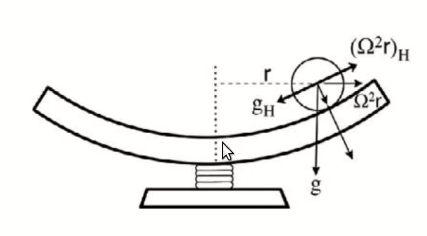
\includegraphics[scale=0.4]{./img/coriolis.png}
	\caption{Figura para ejemplificar la fuerza de \textit{Coriolis}.}
	\label{coriolis}
\end{figure}

Hacemos $\omega = (0,0,\omega)$ y llamamos $v = \dv{*r}{t} = (v_x, v_y, 0)$. Expandiendo el producto vectorial $ \dv{*}{t} (v_x,v_y,0) = (2\omega v_y,-2\omega v_x,0)$ entonces, se tienen ecuaciones diferenciales para las componentes
	\begin{equation}
		\dv{*v_x}{t} = 2\omega v_y, \qquad \dv{*v_y}{t} = -2\omega v_x.
	\end{equation}
Resolviendo las ecuaciones se tiene que 
	\begin{align*}
		v_y (t) &= A \cos{(2\omega t + \theta)} ,\\
		v_x (t) 6= A\sin{(2\omega t + \theta)}
	\end{align*}
Se tomarán como condiciones iniciales $v_x (0) = v_{x0}$ y $v_y (0) = 0$, entonces
	\begin{align}
		v_x (t) &= v_{x0} \sin{(2\omega t + \pi/2)} = \cos{(2\omega t)}, \\
		v_y (t) &= v_{x0} \cos{(2\omega t + \pi/2)} = \sin{(2\omega t)}.
	\end{align}
Integramos para encontrar la posición
	\begin{align}
		x(t) &= \frac{v_{x0}}{2\omega} \sin{(2\omega t)}, \\
		y(t) &= \frac{v_{x0}}{2\omega} \cos{(2\omega t)} - \frac{v_{x0}}{2\omega}.
	\end{align}
Es claro que la trayectoria de la partícula en el sistema estrellado es un círculo.

\subsection{Péndulo de Foucault}
Tomando un péndulo largo y pesado, esto nos da oscilaciones "planas" sin elevación. La fuerza de coriolis es perpendicular al plano de oscilación, es $<0.1\%$ de $mg_e$ y tiene un efecto de precesión del plano de oscilación. Para describir bien esto, nos 'iremos' a un sistema que rota con el plano de oscilación. \\

Introducimos coordenadas en donde el péndulo no precesa. Llamamos $\Omega \vu{z}$ a la \textit{velocidad de precesión del plano}. También llamamos $O'$ al sistema que gira con velocidad $\Omega \vu{z}$, recordamos cómo tomar las derivadas
\begin{equation}
	\dv{r}{t} = \dv{*r}{t} + \omega \times r,\qquad	\dv[2]{r}{t} = \dv[2]{* r}{t} + 2\omega \times \dv{* r}{t} + \omega \times (\omega \times r) + \dv{* \omega}{t} \times r
\end{equation}
Ahora transformaremos, nos trasladaremos del sistema $O^*$ al sistema primado, con lo que se tiene
\begin{equation}
	\dv{*r}{t} = \dv{\prime r}{t} + \Omega \vu{z} \times r, \qquad \dv[2]{*r}{t} = \dv[2]{\prime r}{t} + \Omega \vu{z}\times (\Omega \vu{z} \times r) + 2\Omega \vu{z} \times \dv{\prime r}{t}.
\end{equation}
\dsnote{Son 3 sistemas de coordenadas: El sistema fijo, el sistema estrellado que gira con el planeta y el sistema primado que es el que gira con el péndulo.} Ahora con un poco del álgebra y análisis vectorial\footnote{Identidad BAC-CAB: $\vb{A} \times (\vb{B} \times \vb{C}) = \vb{C}(\vb{A}\cdot \vb{C}) - \vb{C} (\vb{A} \times \vb{B})$} se llega a 
\begin{equation}
	m\dv[2]{\prime r}{t} = \tau + mg_e - 2m (\Omega \vu{z} + \omega) \times \dv{\prime r}{t} - m\Omega \qty[\Omega \vu{z} \cdot r + 2\omega \cdot r]\vu{z} + m(\Omega ^2 + 2\omega \cdot \Omega \vu{z}) r.
\end{equation}
El vector unitario $\vu{z}$ y el vector de posición $r$ están sobre el plano de oscilación. El vector resultante del producto cruz es el único que se sale del plano de oscilación y esto se escapa del objetivo del sistema primado; por ende, tenemos que ajustar la velocidad angular $\Omega$ para que todas las fuerzas involucradas estén dentro del plano de oscilación. Entonces es necesario que $\vu{z} \cdot (\Omega \vu{z} + \omega) = 0$, por lo tanto $\Omega = -\omega \cos{\theta}$ lo que contrarresta la precesión ocacionada por la fuerza de coriolis.





\section{Problema Restringido de los Tres Cuerpos}
Tomaremos el potencial para la masa $m$ del sistema de tres cuerpos
\begin{equation}
	V = -\frac{mM_1 G}{\qty[(x - x_1)^2 + y^2]^{1/2}} - \frac{mM_2 G}{\qty[(x - x_2)^2 + y^2]^{1/2}} - \frac{1}{2} m\omega ^2 \qty(x^2 + y^2),
\end{equation}
donde $\omega$ es la velocidad angular de la órbita circular $M_1$ y $M_2$, la cuál está dada por
	\begin{equation}
		\omega ^2 = \frac{(M_1 + M_2) G}{a^3}.
	\end{equation}
Al igual que las órbitas de fuerza central, nuestro análisis se basa en encontrar los puntos máximos y mínimos de la energía potencial.\\

Para hacer los cálculos más simples se realizará el siguiente cambio de variables.
\begin{align*}
	\xi = \frac{x}{a}, &\qquad \eta = \frac{y}{a}, \\
	\xi _1 = \frac{x_1}{a} = \frac{M_2}{M_1 + M_2}, &\qquad \xi _2 = \frac{x_2}{a} = -\frac{M_1}{M_1 + M_2} = \xi _1 - 1.
\end{align*}
Entonces, reemplazando variables
\begin{equation}
	V = \frac{m (M_1 + M_2) G}{a} \left\{ \frac{\xi _2}{\qty[(\xi - \xi _2)^2 + \eta ^2]^{1/2}} - \frac{\xi _1}{\qty[\qty(\xi - \xi _2)^2 + \eta ^2]^{1/2}} - \frac{1}{2} \qty(\xi ^2 + \eta ^2) \right\} .
\end{equation}

\subsection{Puntos Máximos y Mínimos}
La forma de proceder es tomar las derivadas de $V$ dada por la última ecuación respecto de $\xi$ y $\eta$ e igualarlas a cero. Cone esto llegamos a la siguiente relación
	\begin{equation}
		-\frac{\xi _2 (\xi - \xi _1)}{\abs{\xi - \xi _1}^3} + \frac{\xi _1 (\xi - \xi _2)}{\abs{\xi - \xi _2}^3} - \xi = 0.
	\end{equation}

Haciendo $\eta = 0$ se tienen $3$ puntos $(\xi _A ,0), (\xi _B ,0), (\xi _C ,0)$. Los siguientes dos puntos se encuentran con un poco de álgebra
\begin{align*}
	(\xi - \xi _2)^2 + \eta ^2 &= 1, \\
	(\xi - \xi _1)^2 + \eta ^2 &= 1.
\end{align*}
En donde los puntos $A,B,C$ son puntos silla y $D,E$ son máximos. El resto de la solución es gráfica.





\chapter{Mecánica del Medio Continuo}
\section{Cuerda Vibrante}
Consideraciones generales:
\begin{itemize}
	\item La vibración ocurre en el plano vertical.
	\item La longitud de la cuerda es $l$.
	\item La cuerda está fija en los extremos.
	\item La vibración es pequeña.
	\item Cada punto se mueve verticalmente.
	\item La tensión es constante.
\end{itemize}

Luego de realizar la deducción se tiene la ecuación de onda
\begin{equation}
	\laplacian{p} - \frac{1}{c^2} \pdv[2]{p}{t} = 0.
\end{equation}

Resolviendo la ecuación por separación de variables se tienen las siguientes ecuaciones
\begin{align}
	\Theta (t) &= A \cos{\omega t} + B \sin{\omega t}. \qquad \textbf{Ecuación de Helmholtz} \\
	X(x) &= C_x \cos{k_x x} + D_x + \sin{k_x x}, \\
	Y(y) &= C_y \cos{k_y y} + D_y + \sin{k_y y}, \qquad \textbf{Soluciones Espaciales} \\
	Z(z) &= C_z \cos{k_z z} + D_z + \sin{k_z z}.
\end{align}

Donde la constante de $z$ depende de las otras dos, y esta relación es
\begin{equation}
	\frac{\omega ^2}{c^2} = k_x ^2 + k_y ^2 + k_z ^2.
\end{equation}
Luego de aplicar las condiciones de frontera 
\begin{equation}
	p = \qty(A \cos{\omega _{lmn} t} + B \sin{\omega _{lmn} t}) \cos{\frac{l\pi x}{L_x}} \cos{\frac{m\pi y}{L_y}} \cos{\frac{n\pi z}{L_z}}.
\end{equation}

\begin{enumerate}
	\item Las frecuencias $\omega _{lmn}$ no son múltiplos enteros de una misma cantidad, como en el caso de la cuerda. Esto es importante porque es la razón por la cual una cuerda puede producir notas musicales.
\end{enumerate}

\subsection{Ondas Viajeras}
Luego de encontrar la solución a la ecuación de onda en una dimensión
\begin{equation}
	u(x,t) = A \sin{\frac{n\pi x}{l}} \cos{\frac{n\pi ct}{l}} + \sin{\frac{n\pi x}{l}} \sin{\frac{n\pi ct}{l}}.
\end{equation}


\subsubsection{Ondas Viajeras y Estacionarias}
\begin{equation}
	\underbrace{B \sin{\frac{n\pi x}{l}} \sin{\frac{n\pi ct}{l}}}_{\text{ONda Estacionaria}} = \underbrace{\frac{B}{2} \cos{\frac{n\pi}{l} (x - ct)}}_{\text{Onda Viajera a la }\to} - \underbrace{\frac{B}{2} \cos{\frac{n\pi}{l} (x + ct)}}_{\text{Onda Viajera a la } \leftarrow}.
\end{equation}

\begin{tcolorbox}
	Para formar una onda estacionaria tenemos que superponer dos ondas
viajeras con igual amplitud y que se muevan en direcciones opuestas con
igual velocidad. 
\end{tcolorbox}


\section{Equilibrio de Fluidos}
\subsection{Fuerzas de Volumen}
Fuerza de volumen $f$, es la traducción común de \textit{body force}. Es la fuerza que experimenta un fluido por unidad de volumen, de tal forma que un elemento de volumen $\dd{V}$ experimenta una fuerza dada por $f\dd{V}$. El ejemplo más común es la fuerza de volumen ejercida por la gravedad, que está dada como $f = \rho g$ donde $\rho$ es la densidad del fluido.

\subsection{Relación entre Presión y Energía Potencial}
Encontrar la presión dentro de un fluido en equilibrio sabiendo la fuerza de volumen $f(r)$ es equivalente a encontrar la \textbf{energía potencial} para una fuerza $F(r)$. Primero verificamos que  $\curl{f}$ sea cero en todo el fluido. Luego tomamos un punto  $r_1$ en donde la presión es conocida y utilizamos la expresión
	\begin{equation}
		p(r) = p_1 + \int _{r_1} ^r f\cdot \dd{r}.
	\end{equation}
que es una integral de línea a lo largo de una trayectoria. Si $\curl{f} = 0$ implica que $f$ se puede expresar como el gradiente de una cantidad. De la expresión entre la fuerza de volumen $f$ y la presión $p$ es
	$$ f = \grad{p}. $$
En el caso de fuerza de gravedad, sabemos que ésta apunta de arriba hacia abajo. El gradiente de la presión apunta en la misma dirección ya que la presión aumenta de arriba hacia abajo.



\section{Cinemática de Fluidos}
Se tienen dos puntos de vista
\begin{itemize}
	\item \textbf{Lagrangiano:} 
	\begin{itemize}
		\item Seguir el movimiento de un elemento de fluido.
		\item Dada su posición inicial $\to$ posición futura.
		\item Como un sistema de partículas, forma en la que describimos la cuerda.
	\end{itemize}
	\item \textbf{Euleriano:}
	\begin{itemize}
		\item Establecer densidad y velocidad para cada punto e instante.
		\item El fluido se describe con la densidad $\rho (x,y,z,t)$ y la velocidad $v(x,y,z,t)$.
		\item Centramos la atención en lo que sucede en un punto fijo en lugar de seguir a las partículas en su trayectoria.
	\end{itemize}
\end{itemize}


\subsection{Dos Tipos de Razones de Cambio}
Desarrollando un poco el diferencial de presión
\begin{equation}
	\boxed{ \dv{p}{t} = \pdv{p}{t} + v\cdot \grad{p}. }
\end{equation}

\subsection{Fluido Incompresible}
Estudiando un poco la divergencia se tiene
\begin{equation}
	\dv{t} (\delta V) = (\div{v}) \delta V.
\end{equation}
Un caso importante a considerar es cuando $\div{v} = 0$, en cuyo caso vemos de la derivada del volumen es igual a cero, o bien que $\delta V$ se mantiene constante. En otras palabras, decimos que el fluido es \textbf{incompresible}.

\begin{tcolorbox}
	Un fluido es incompresible si cumple con $\div{v} = 0$.
\end{tcolorbox}
Esta condición se cumple cuando el fluido es un líquido. Un gas se expande y se contrae, pero en ciertos casos se puede considerar incompresible también. Sin embargo, recordemos también que ningún objeto es totalmente líquido.

\subsection{Masa}
Suponiendo que la masa de un elemento de volumen es constante $\delta m = \rho \delta V$. Derivando respecto al tiempo y desarrollando $\dv{t} \delta m$
\begin{equation}
	\pdv{\rho}{r} + \div{\rho v} = 0,
\end{equation}
A lo que se le conoce como \textbf{ecuación de continuidad} y expresa e hecho de que la masa de cada elemento de volumen es constatne, por lo tanto la masa total de todo el fluido también es constante. En otras palabras, la masa se conserva.

\subsection{Voriticidad}
Es el elemento proyectado en la dirección de un vector unitario $\vu{n}$
\begin{equation}
	\text{Vorticidad} = \vu{n} \cdot \qty(\curl{v}).
\end{equation}
Si integramos la vorticidad en una superficie con vector normal, utilizando el teorema de Stokes, en donde si las integrales son cero podemos decir que la vorticidad es cero y esto nos dice que el fluido es \textbf{irrotacional}.

\subsection{Ecuacion de Movimiento para un Fluido Ideal}
\begin{equation}
	\pdv{v}{t} = v\cdot \grad{v} + \frac{1}{\rho} \grad{\rho} = \frac{f}{p}.
\end{equation}
Si $\rho = \rho (p)$ entonces el fluido es homogeneo.


\subsection{Ley de Conservación}
Vamos a partir de la ecuación de continuidad, la cual también le podemos llamar \textbf{ley de conservación de masa}. 

\begin{equation}
	\dv{t} \underbrace{\iiint _V \rho \dd{V}}_{\text{masa}} + \underbrace{\iint _S \vu{n} \cdot v \rho \dd{S}}_{\text{flujo de masa}} = 0.
\end{equation}
Esto dice que la forma de una ley de conservación es
\begin{equation}
	\dv{t} X + \text{flujo de } X = 0,
\end{equation}
donde $X$ es cualquier cantidad física qeu nos interese, por ejemplo: masa, momentum, energía, momentum angular, etc. Una forma generalizada es con la ecuación anterior es igual a $Q$, a la cual se le llama \textbf{fuente} o \textbf{sumidero}.\\

De esto y de la fuerza de volumen podemos concluir que 
\begin{equation}
	\frac{1}{2} \rho v^2 + p - \rho \mathcal{G} = \text{cte}.
\end{equation}

\subsection{Flujo Estacionario}
\begin{itemize}
	\item Velocidad, densidad, presión, fuerzas de volumen son constantes en el tiempo.
	\item No cambian en el tiempo pero si en e espacio.
	\item Las derivadas $\pdv{t}$ son cero.
	\item La expresión $\dv{t} = \pdv{t} + v\cdot \nabla \, \to \, \dv{t} = v\cdot \nabla$.
\end{itemize}






\chapter{Mecánica Lagrangiana y Hamiltoniana}

\section{Introducción}
¿Por qué esto no es satisfactorio en la física moderna?
\begin{enumerate}
	\item ''Oscurece'' algunas características de la dinámica de un sistema.
	\item No está clara la relación entre las leyes de Newton y la Mecánica Cuántica.
	\item Es dificil trabajar con sólidos.
\end{enumerate}

Identificar estructuras y simetrías en los sistemas. Sistemas locales: QED, QCD, Débiles.


\subsection{Mecánica Newtoniana}
Segunda ley de Newton
\begin{equation}
	\vec{F} = m\vec{a} \longrightarrow \vec{F} (\vec{r}, \dot{\vec{r}}) = \dot{\vec{p}}.
\end{equation}
donde $\dot{m} = 0$. Si conocemos $\vec{r}$ y $\dot{\vec{r}}$ en un tiempo $t=t_o$, integrando se encuentra $\vec{r} (t)$.

\subsection{Marco de Referencia Inercial}
Es en el que una partícula con masa constante viaja en una línea recta.
\begin{equation}
	\vec{r} = \vec{r}_o + \vec{v} t.
\end{equation}
Si $S$ es un marco de referencia inercial se tienen $10$ transformaciones lineales independientes $S \to S\prime$ también es un M.R. inercial.
\begin{itemize}
	\item 3 Rotaciones: $\vec{r}' = O \vec{r}$ donde $O$ es una matriz $3\times 3$ ortogonal.
	\item 3 Traslaciones: $\vec{r}' = \vec{r} + \vec{c}$ donde $\vec{c}$ es un vector constante.
	\item 3 Boost: $\vec{r}' = \vec{r} + \vec{u} t$ donde $\vec{u}$ es una velocidad constante.
	\item 1 Traslaciones Temporales: $t' = t + c$ donde $c$ es real y constante.
\end{itemize}
Las leyes de Newton son invariantes ante este grupo de transformaciones: \textbf{Grupo Galileano.}


\subsection{Momento Angular}
\begin{equation}
	\vec{L} = \vec{r} \times \vec{p}
\end{equation}
Medimos respecto a un punto en partícular.
\begin{equation}
	\vec{\tau} = \dot{\vec{L}}
\end{equation}

\subsubsection{Leyes de Conservación}
\begin{itemize}
	\item Si $\vec{F} = 0$ entonces $\vec{p}$ es constante.
	\item Si $\vec{\tau} = 0$ entonces $\vec{L}$ es constante.
\end{itemize}

\subsection{Energía}
Energía cinética $T = \frac{1}{2} m \dot{\vec{r}} \cdot \dot{\vec{r}}$
\begin{equation}
	\dv{T}{t} = \vec{F} \cdot \dot{\vec{r}},
\end{equation}
entonces
\begin{equation}
	W = \int _{r_1} ^{r_2} \vec{F} \cdot \dd{\vec{r}}.
\end{equation}

\textbf{Fuerzas Conservativas:} El trabajo realizado es independiente de la trayectoria. Y para una trayectoria cerrada
\begin{equation*}
	\oint \vec{F} \cdot \dd{r} = 0 \quad \Leftrightarrow \quad \curl{\vec{F}} = 0.
\end{equation*}
Por lo que se puede escribir $\vec{F} = -\grad{V(r)}$. \\

Energía cinética de un sistema $T = \frac{1}{2} \sum _i m \dot{\vec{r}}_i ^2$ y tomando $\vec{r} _i = \vec{R} + \vec{\rsim}$
\begin{equation}
	T = \frac{1}{2} M \dot{\vec{R}}^2 + \frac{1}{2} \sum _i \dot{\vec{\sim}},
\end{equation}
como en el caso de una sola partícula
\begin{equation}
	T(t_2) - T(t_1) = \sum _i \int \vec{F} _i ^{ext} \cdot \dd{\vec{r}_i} + \sum_{i\neq j} \int \vec{F} _{ij} \cdot \dd{\vec{r}_i}.
\end{equation}

\begin{itemize}
	\item Fuerzas externas conservativas: $\vec{F} _i ^{ext} = -\grad{V_i} \qty(\vec{r}_1, \ldots ,\vec{r}_N)$.
	\item Fuerzas internas conservativas: $\vec{F}_{ij} = -\nabla _i V_{ij} (\vec{r}_1 ,\ldots ,\vec{r}_N)$. $\vec{F} _{ij} = -\vec{F}_{ij}$ $\to$ $V_{ij} = V_{ji}$ entonces $V_{ij} (\vec{r}_1 ,\ldots ,\vec{r}_N) = V_{ij} (\abs{\vec{r}_1 - \vec{r}_j})$.  
\end{itemize}

\begin{equation}
	T(t_2) - T(t_1) = -\sum _i \int \nabla _i V_i (\vec{r}_i) \cdot \dd{r}_i - \sum _{i\neq j} \int \nabla _i V_{ij} (r_1 ,\ldots, r_N) \cdot \dd{r}_i.
\end{equation}


\section{Generalidades}
\subsection{Principio Variacional y Ecuación de Lagrange}
Movimiento de un sistema. Coordenadas generalizadas: $q_1 ,q_2, \ldots, q_n$, espacio de $n$ dimensiones \dsnote{Espacio de Configuración}\footnote{Cada punto de la curva en el espacio de configuración es un instante en la configuración del sistema.}. 

\subsection{El Principio de Hamilton (Principio de Mínima Acción)}
El movimiento del sistema de un tiempo $t_1$ a un tiempo $t_2$ es tal que la acción
	\begin{equation}
		I = \int _{t_1} ^{t_2} \lagran \dd{t}
	\end{equation}

donde $\lagran$ es el Lagrangiano $T - V$, tiene un valor estacionario para el movimiento.
\begin{align*}
	\delta I &= 0, \\
	\delta I &= \delta \int _{t_1} ^{t_2} \lagran (q_1 ,\ldots ,q_n ,\dot{q}_1 ,\ldots ,\dd{q}_n ;t) \dd{t} = 0.
\end{align*}
Principio de Hamilton es suficiente para derivar las ecuaciones de movimiento.

\subsection{Cálculo de Variaciones}
\dsnote{''Repaso'' de algo que nunca se vió bien xd.}
Consideremos un problema de $1$ dimensión $f(y,\dot{y} ,x)$ donde $y = y(x)$, $\dot{y} = \dv{y}{x}$, $[x_1 ,x_2]$. Todo esto es por $\delta J = 0$, entonces
	\begin{equation}
		J = \int _{x_1} ^{x_2} f(y,\dot{y},t) \dd{x}.
	\end{equation}
Donde $y(x,\alpha)$ son posibles trayectorias y $y(x,0)$ es la trayectoria correcta. Podemos escribir $y(x,\alpha) = y(x,0) + \alpha \eta (x)$, donde $\eta (x)$ tiene que ser $0$ en $x_1$ y $x_2$. 
\begin{align*}
	J(\alpha) = \int _{x_1} ^{x_2} f\qty(y(x,\alpha), \dot{y} (x,\alpha), x) \dd{x}, \\
	\qty(\dv{J}{\alpha}) _{\alpha = 0} = 0. \qquad \text{Para un punto estacionario.}
\end{align*}

Derivando
\begin{equation}
	\dv{J}{\alpha} = \int _{x_1} ^{x_2} \qty(\pdv{f}{y} \pdv{y}{\alpha} + \pdv{f}{\dot{y}} \pdv{\dot{y}}{\alpha}) \dd{\alpha}
\end{equation}
Considerando solo la segunda derivada al realizar integración por partes
\begin{equation}
	\int _{x_1} ^{x_2} \pdv{f}{\dot{y}} \pdv{\dot{y}}{\alpha} \dd{x} = \int _{x_1} ^{x_2} \pdv{f}{\dot{y}} \pdv[2]{y}{\alpha}{x} \dd{x} = - \int _{x_1} ^{x_2} \dv{x} \qty(\pdv{f}{\dot{y}}) \pdv{y}{\alpha} \dd{x}.
\end{equation}

\begin{align*}
	\dv{J}{\alpha} &= \int _{x_1} ^{x_2} \qty(\pdv{f}{y} - \dv{x} \pdv{f}{\dot{y}}) \pdv{y}{\alpha} \dd{x} \\
	&\int _{x_1} ^{x_2} \qty(\pdv{f}{y} - \dv{x} \pdv{f}{\dot{y}}) \qty(\pdv{y}{\alpha})_{\alpha = 0} \dd{x} = 0 \qquad \text{Condición puntos estacionarios} \\
	\text{Recordemos } &\quad y(x,\alpha) = y(x,0) + \alpha \eta (x).
\end{align*}

\subsubsection{Lema: }
\begin{equation}
	\int _{x_2} ^{x_1} M(x) \eta (x) \dd{x} = 0
\end{equation}
para $\eta (x)$: función arbitraria y continua (hasta la segunda derivada). $M(x)$ se desvanece en el intervalo $(x_1,x_2)$
\begin{equation}
	\pdv{f}{y} - \dv{x} \qty(\pdv{f}{\dot{y}}) = 0
\end{equation}
la cantidad diferencial
	\begin{equation}
		\qty(\pdv{y}{\alpha})_{\alpha = 0} \dd{\alpha} \equiv \delta y
	\end{equation}
variación infinitesimal de la trayectoria variada respecto de la trayectoria correcta. La variación de $J$
\begin{equation}
	\qty(\pdv{J}{\alpha})_{\alpha = 0} \dd{\alpha} \equiv \delta J
\end{equation}
entonces
\begin{equation}
	\delta J = \int _{x_1} ^{x_2} \qty(\underbrace{\pdv{f}{y} - \dv{x} \pdv{f}{\dot{y}}}_{=0}) \delta y \dd{x} = 0
\end{equation}

\subsection{Principio de Hamilton y Ecuación de Lagrange}
\begin{equation}
	\delta J = \int _1 ^2 f(y_1 (x), \ldots; \dot{y} _1 (x), \ldots; x) \dd{x}
\end{equation}
Lo de $y_i(x,\alpha)$ se cumple para todas las $i$, donde lo que nos interesa son las $y_i (x,0)$, sabiendo que $\eta _i (x)$ se desvanecen en los extremos. Realizando el mismo análisis que se realizó en la subsección anterior, se llega a 
	\begin{equation}
		\boxed{ \pdv{f}{y_i} - \dv{x} \pdv{f}{\dot{y}_i} = 0 }
	\end{equation}
En donde si se tienen $N$ partículas, implica tener $n = 3N$ coordenadas. Cambiando de coordenadas
\begin{equation}
	\boxed{ \dv{t} \pdv{\lagran}{\dot{q}_i } - \pdv{\lagran}{q_i} = 0 }
\end{equation}
a lo que se conoce como \textbf{Ecuación de Lagrange}.

\subsection{Restricción en las Coordenadas Generalizadas}

\subsubsection{Restricciones Holonómicas}
\begin{equation}
	f(x_A ,t) = 0
\end{equation}
$\alpha = 1,2,\ldots ,N-n$ con $N$ número total de coordenadas y $n$ número de grados de libertad. Por ejemplo: para $M$ partículas, se tienen $3M$ ecuaciones, que es lo mismo que $3M = N$ coordenadas, y $n$ ecuaciones/grados de libertad.
\paragraph{Multiplicadores de Lagrange} $x_A = x_A (q_1, \ldots ,q_n)$, $N - n$ nuevos grados dinámicos de libertad, $\lambda _\alpha (t)$. Definimos el nuevo lagrangiano $\lagran ^\prime = \lagran (x^A, \dot{x}^A) + \lambda _\alpha f_\alpha (x^A ,t)$
\begin{equation}
	\underbrace{\dv{t} \pdv{\lagran}{\dot{x}_A} - \pdv{\lagran}{x_A}}_{\text{La ecuación de movimiento sin restricciones}} = \underbrace{\lambda _\alpha \pdv{f_\alpha}{x_A}}_{Restricciones en el sistema}
\end{equation}

\begin{teorema}
	\begin{equation}
		\lagran [q_i, \dot{q}_i,t] = \lagran [x^A(q_i ,t), \dot{x}^A (q_i ,\dot{q}_i ,t),t]
	\end{equation}
	Imponer una restricción $\lagran ^\prime = \lagran + \lambda _\alpha f_\alpha$
	\begin{equation}
		\boxed{ \dv{t} \pdv{\lagran}{\dot{q}_i} - \pdv{\lagran}{q_i} = \lambda _\alpha \pdv{f_\alpha}{q_i}, } \qquad \to \qquad \boxed{ \pdv{f_\alpha}{q_i} = 0. }
	\end{equation}
\end{teorema}
\paragraph{Resumen} Un sistema descrito por $N$ coordenadas generalizadas $q_i$
\begin{align*}
	\lagran (q_i ,\dot{q}_i ,t) \to \dv{t} \pdv{\lagran}{\dot{q}_i} - \pdv{\lagran}{q_i} = 0.
\end{align*}
\begin{itemize}
	\item Momento conjugado de $q_i$ $/$ momento canónico
	\begin{align}
		p_i &= \pdv{\lagran}{\dot{q}_i} \\
		\boxed{ \dot{p}_i = \pdv{\lagran}{q_i}. }
	\end{align}
\end{itemize}

\subsection{Teorema de Noether}
\begin{definition}
	$F(q_i, \dot{q}_i, t)$ constante de movimiento, cantidad conservada.
	\begin{equation}
		\dv{F}{t} = 0 \qquad \sum _{j=1} ^N \qty(\pdv{F}{q_j} \dot{q}_j + \pdv{F}{\dot{q}_i} \ddot{q}_i) + \pdv{F}{t} = 0
	\end{equation}
	para $q_i$ que satisface la ecuación de movimiento. Si $\lagran$ no depende explícitamente del tiempo.
	\begin{equation}
		H = \sum _j \dot{q}_j \pdv{\lagran}{\dot{q}_j} - \lagran = \text{cte}.
	\end{equation}
	Derivando el Hamiltoniano respecto al tiempo se supone $\pdv{\lagran}{q_j} = 0$ solo para algunas $q_j$.
	\begin{align*}
		p_j &= \pdv{\lagran}{\dot{q}_j} \\
		\dv{p_j}{t} &= \dv{t} \pdv{\lagran}{\dot{q}_j} = \pdv{\lagran}{q_j} = 0.
	\end{align*}
	Mapeo de los parametros $q_j = Q_j (s,t)$ $s\in \R$ De modo que $q_j (t) = Q_j (0,t)$, se dice que esta transformación es una simetría contínua del $\lagran$.
	\begin{equation}
		\pdv{\lagran}{s} (Q_j (s,t), \dot{Q}_j (s,t)) = 0.
	\end{equation}
	El teorema de Noether: Para cada una de estas simetrías hay una cantidad conservada.
	\begin{align*}
		\pdv{\lagran}{s} &= \pdv{\lagran}{Q_j} \pdv{Q_j}{s} + \pdv{\lagran}{\dot{Q}_j} \pdv{\dot{Q}_j}{s} \\
		\eval{\pdv{\lagran}{\dot{q}_j} \pdv{Q_j}{s}}_{s=0} &= \text{cte}.
	\end{align*}
	\begin{itemize}
		\item Invarianza de $\lagran$ ante traslaciones: Se conserva el momentum lineal.
		\item Invarianza de $\lagran$ ante rotaciones: Se conserva el momentum angular.
		\item Homogeneidad en el tiempo: Conservaciń de la energía.
	\end{itemize}
\end{definition}

\section{Formalismo de Hamilton}

\subsection{Ecuación de Hamilton}
\begin{equation}
	H(q_i, p_i, t) = \sum _{i=1} ^n p_i q_i - \lagran (q_i,p_i,t)
\end{equation}
con $\pdv{\lagran}{\dot{q}_i} = p_i$, ahora veamos la variación de $H$
\begin{equation}
	\dd{H} = (\dd{p}_i) \dot{q}_i - \pdv{\lagran}{q_i} \dd{q}_i - \pdv{\lagran}{t} \dd{t}
\end{equation}
Esto lo podemos escribir como
\begin{align}
	\dd{H} &= \pdv{H}{q_i} \dd{q}_i + \pdv{H}{p_i} \dd{p}_i + \pdv{H}{t} \dd{t} \\
	\boxed{\dot{p}_i = -\pdv{H}{q_i}} &\qquad \boxed{\dot{q}_i = \pdv{H}{p_i}} \qquad \boxed{-\pdv{\lagran}{t} = \pdv{H}{t}}.
\end{align}




\subsection{Teorema de Liuville}







\subsection{Brakets de Poisson}
Teniendo $f(p,q)$, $g(q,p)$ se define un braket de poisson
\begin{equation}
	\{ f,g \} = \pdv{f}{q_i} \pdv{g}{p_i} - \pdv{f}{p_i} \pdv{g}{q_i}.
\end{equation}
Con las siguientes propiedades
\begin{itemize}
	\item $\{ f,g \} = -\{ g,f \}$.
	\item Linealidad: $ \{ \alpha f + \beta g, h \} = \alpha \{ f,h \} + \beta \{ g,h \} $.
	\item Leibniz rule: $\{ fg,h \} = f\{ g,h \} + \{ f,h \} g$.
	\item Identidad de Jacobi: $\{ f,\{ g,h\} \} + \{ g,\{ h,f\} \} + \{ h,\{ f,g\} \} = 0$.
	\item Y por ultimo, para una función:
		\begin{equation}
			\dv{f}{t} = \{ f,H \} + \pdv{f}{t}.
		\end{equation}
\end{itemize}




\subsection{Transformaciones Canónicas}
Tomando $\mathcal{J} _{ij} \equiv \pdv{y_i}{x_j}$, para que las ecuaciones de Hamilton queden invariantes
	\begin{equation}
		\boxed{ \mathcal{J} J \mathcal{J} ^T = J.} \qquad \text{Transformación Canónica.}
	\end{equation}

\begin{teorema}
	Los brackets de Poisson son invariantes ante transformaciones canónicas. Si los brackets de Poisson preservan la estructura:
	\begin{equation}
		\{ Q_i,Q_j \} = 0 \qquad \{ P_i,P_j \} = 0 \qquad \{ Q_i,p_j \} = \delta _{ij}
	\end{equation}
	la transformación es canónica.
\end{teorema}
















\chapter{Cuerpo Rígido}
\section{Generalidades}
$N$ puntos en donde la distancia entre ellos está fijo $\abs{r_i - r_j} = $constante en el límite continuo $\sum _i m_i \to \int \dd{r} \rho (r)$. En donde se tienen $6$ grados de libertad $3$ traslaciones y $3$ rotaciones. Ahora definimos $\{ \vu{\overset{\sim}{e}}_a \}$ es el marco de referencia del espacio y $\{ \vu{e}_a \}$ es el marco de referencia del cuerpo rígido. En donde los productos internos entre elementos de los marcos de referencia cumplen con la ortonormalidad. \\

Espacio de configuración, $C$, matrices $3\times 3$ ortogonales especiales SO($3$).

\subsection{Velocidad Angular}
Teniendo $\vec{r} (t) = \overset{\sim}{r} _a (t) \vu{\overset{\sim}{e}_a} = r_a \vu{e} _a (t)$, ahora $r_a \vu{e} _a (t) = r_a R_{ab} (t) \vu{\overset{\sim}{e}} _b$, donde $R_{ab}$ son elementos de una matriz. Derivamos respecto al tiempo con lo que analizamos tanto los vectores posición como la base $\dv{\vu{e}_a (t)}{t} = \dv{R_{ab}}{t} R_{cd} \vu{e}_a = \omega _{ac} \vu{e}_c$ y por facilidad definimos un objeto con un solo índice $\omega _a = \frac{1}{2} \varepsilon _{abc} \omega _{bc}$\footnote{Donde $\varepsilon _{abc}$ es conocido como el símbolo de Levi Civita.}.
\begin{equation}
	\dv{\vu{e}_a}{t} = \vec{\omega} \times \vu{e}_a.
\end{equation}
con $\omega$ velocidad angular instantánea en el marco de referencia del cuerpo rígido.



\subsection{El Tensor de Inercia}
\begin{equation}
	T = \frac{1}{2} \sum _i m_i \dot{\vec{r}}_i ^2
\end{equation}
usando $\dot{\vec{r}} = \vec{\omega} \times \vec{r}$
\begin{equation}
	T = \frac{1}{2} \sum _i m_i (\vec{\omega} \times \vec{r}_i) \times (\vec{\omega} \times \vec{r} _i)
\end{equation}
usando y desarrollando una identidad para los producto cruz e interno, por lo que se tiene que
\begin{equation}
	T = \frac{1}{2} \omega _a I_{ab} \omega _b,
\end{equation}
donde $I_{ab} = \sum_i m_i \qty[\vec{r}_i \cdot \vec{r}_i \delta _{ab} - (\vec{r}_i)_a (\vec{r}_i)_b]$ donde $I_{ab}$ es el tensor de inercia, es simétrico
\begin{equation}
	I = \int \dd ^3 r \rho (\vec{r}) \mqty( y^2 + z^2 & -xy & -xz \\ -xy & x^2 + z^2 & -yz \\ -xz & -yz & y^2 + x^2 )
\end{equation}

$I^\prime = OIO^T$ donde $I^\prime$ es diagonal $I^\prime = \mqty(\dmat{I_1,I_2,I_3})$ con $I_a$ son los momentos de inercias principales.

\begin{tcolorbox}
	Propiedades del cuerpo rígido están dadas por su masa, su momento de inercia y sus ejes principales.
\end{tcolorbox}

$I_a$ es real y positivo.
\begin{equation}
	I_{ab} c^a c^b = \sum _i \qty(r_i ^2 c^2 - (\vec{r}_i \cdot \vec{c})^2) \geq 0.
\end{equation}
Si $\vec{c}$ es autovector de $I$, $I_{ab} c_a c_b = I_a \abs{\vec{c}}^2$, $I_a > 0$.

\begin{teorema}
	\textbf{Teorema de Ejes Paralelos: (Forma tensorial)}
	\begin{equation}
		\boxed{ \qty(I_c)_{ab} = \qty(I_{cm})_{ab} \qty(c^2 \delta _{ab} - c_a c_b)M }.
	\end{equation}
\end{teorema}


\subsubsection{Ecuaciones de Euler}
\begin{align*}
	I_1 \dot{\omega}_1 + \omega _2 \omega _3 (I_3 - I_2) &= 0, \\
	I_2 \dot{\omega}_2 + \omega _1 \omega _3 (I_1 - I_3) &= 0, \\
	I_3 \dot{\omega}_3 + \omega _1 \omega _2 (I_2 - I_1) &= 0.
\end{align*}


















































































%%%%%